\section{Results}
\label{sec:results}

The results for the electron and muon channels are presented separately.
Assuming lepton universality, we combine our measurements in the different lepton
decay modes. The electron and muon channels are combined by calculating an
average value weighted by the combined statistical and systematic uncertainties,
taking into account the correlated uncertainties.
For the cross-section measurements, correlations are only numerically
relevant for theoretical uncertainties,
including the PDF uncertainties on the acceptance values. For the cross
section ratio measurements, the correlations
of lepton efficiencies are taken into account in each lepton channel.
%with other experimental uncertainties assumed
%uncorrelated;
In the combination of lepton channels, fully
correlated theoretical uncertainties are assumed for the acceptance factor,
with other uncertainties assumed uncorrelated. The luminosity uncertainty
cancels exactly in the cross-section ratios.

We separate the quoted uncertainties in the statistical contribution (stat.), the
contribution due to experimental systematic uncertainties (syst.), which have been
described in Sec.~\ref{subsec:ELEsystematics} and~\ref{sec:muonSyst}, 
the total theoretical uncertainty (th.), described in Sec.~\ref{sec:theory}, which affects
the acceptance determinations, and the uncertainty on the integrated luminosity (lumi.), which 
cancels in the measurements of cross section ratios.

The NNLO predictions of the total cross sections and their ratios were estimated
using {\sc fewz} and the MSTW 2008 PDF. The uncertainties, at 68$\%$ CL, include
contributions from the strong coupling $\alpha_S$~\cite{Martin:2009bu,GWatt}, the choice of heavy quark masses
(charm and bottom quarks)~\cite{Martin:2009hq} as well as neglected higher-order corrections
beyond NNLO, by allowing the renormalization and factorization scales to vary in a similar way to that
described in Section~\ref{sec:theory}.

The following cross sections for inclusive $\Wo$ production are measured:
{\footnotesize
\begin{eqnarray*}
 \WEISIGBR , \\
 \WMISIGBR , \\
 \WLISIGBR .
\end{eqnarray*}
}%
The corresponding NNLO prediction is $\THEORYSIGBRWI$.
The results for charge-specific $\Wo$ production are
{\footnotesize
\begin{eqnarray*}
 \WEPSIGBR , \\
 \WMPSIGBR , \\
 \WLPSIGBR ,
\end{eqnarray*}
}%
and
{\footnotesize
\begin{eqnarray*}
 \WEMSIGBR , \\
 \WMMSIGBR , \\
 \WLMSIGBR .
\end{eqnarray*}
}%
The NNLO predictions for these cross sections are $\THEORYSIGBRWP$
for~$\Wp$ and $\THEORYSIGBRWM$ for~$\Wm$.
The following cross sections for inclusive $\Zo$ production are measured:
{\footnotesize
\begin{eqnarray*}
 \ZEESIGBR , \\
 \ZMMSIGBR , \\
 \ZLLSIGBR .
\end{eqnarray*}
}%
The reported $\Zo$ cross sections correspond to the
invariant mass range $60 < m_{\ell^+\ell^-} < 120~\GeV$, and
are corrected for the kinematic acceptance but not for $\gamma^*$ exchange.
The NNLO prediction for $\Zo$ production is $\THEORYSIGBRZ$.

\par
The ratio of cross sections for $\Wo$ and $\Zo$ production is
\begin{displaymath}
  \frac{\sigma_{\Wo}}{\sigma_{\Zo}} =
  \frac{N_{\Wo}}{N_{\Zo}} \,
  \frac{\epsilon_{\Zo}}{\epsilon_{\Wo}} \,
  \frac{A_{\Zo}}{A_{\Wo}} \,,
\end{displaymath}
where $A_{\Zo}$ and $A_{\Wo}$ are the acceptances for Z and W selections, respectively.
For the ratio measurement in the muon channel, the signal yield determined by the 
simultaneous fit $\NZtomumu$ is used in place of the ratio $N_{\Zo}/\epsilon_{\Zo}$.
The two different decay channels
are combined by assuming fully correlated uncertainties for the
acceptance factors, with other uncertainties assumed uncorrelated.
The resulting ratios are:
\begin{eqnarray*}
  \RESRATWZE , \\
  \RESRATWZM , \\
  \RESRATWZL . \\
\end{eqnarray*}
The NNLO prediction for this ratio is $\THEORYRATIOWZ$,
in good agreement with the measured value.

The ratio of cross sections for $\Wp$ and $\Wm$ production is given by
\begin{displaymath}
  \frac{\sigma_{\Wp}}{\sigma_{\Wm}} =
  \frac{N_{\Wp}}{N_{\Wm}} \,
  \frac{\epsilon_{\Wm}}{\epsilon_{\Wp}} \,
  \frac{A_{\Wm}}{A_{\Wp}} \,,
\end{displaymath}
where $A_{\Wp}$ and $A_{\Wm}$ are the acceptances for $\Wp$ and $\Wm$, respectively.
The two different decay channels are combined by assuming fully correlated uncertainties for the acceptance
factors, with other uncertainties assumed uncorrelated.  This results
in the measurements:
\begin{eqnarray*}
  \RESRATWWE , \\
  \RESRATWWM , \\
  \RESRATWWL . \\
\end{eqnarray*}
The NNLO prediction for this ratio is $\THEORYRATIOWW$, which agrees
with the presented measurement.

Summaries of the measurements are given in Figs.~\ref{fig:WZ_LEPstylePlots},
 \ref{fig:WPM_LEPstylePlots}, and~\ref{fig:R_LEPstylePlots},
illustrating the consistency of the measurements
in the electron and muon channels, as well as confirming the
theoretical predictions computed at the NNLO in QCD with state-of-the-art
PDF sets. For each reported measurement, the statistical error is represented in black and
the total experimental uncertainty, obtained by adding in quadrature the statistical and
systematic uncertainties, in dark blue. For the cross-section measurements, the luminosity
uncertainty is added to the experimental uncertainty, and is represented in green.
The dark-yellow vertical line represents the theoretical prediction, and the light-yellow
vertical band is the theoretical uncertainty, interpreted as a 68$\%$ confidence interval,
as described earlier.

The ratios of the measurements to the theoretical
predictions are listed in Table~\ref{tab:RatioCMSTHY}
and displayed in Fig.~\ref{fig:RatioCMSTHY}. The experimental
uncertainty (exp.) is computed as the sum in quadrature of the
statistical uncertainty and the systematic uncertainties aside
from the uncertainty on the integrated luminosity and the
theoretical uncertainties associated with the acceptance.
The theoretical uncertainty (th.) is computed by adding in
quadrature the theoretical uncertainties of the acceptance (or the
acceptance ratio) and the NNLO prediction, assuming that they are
uncorrelated.


\begin{figure}[htbp]
\begin{center}
  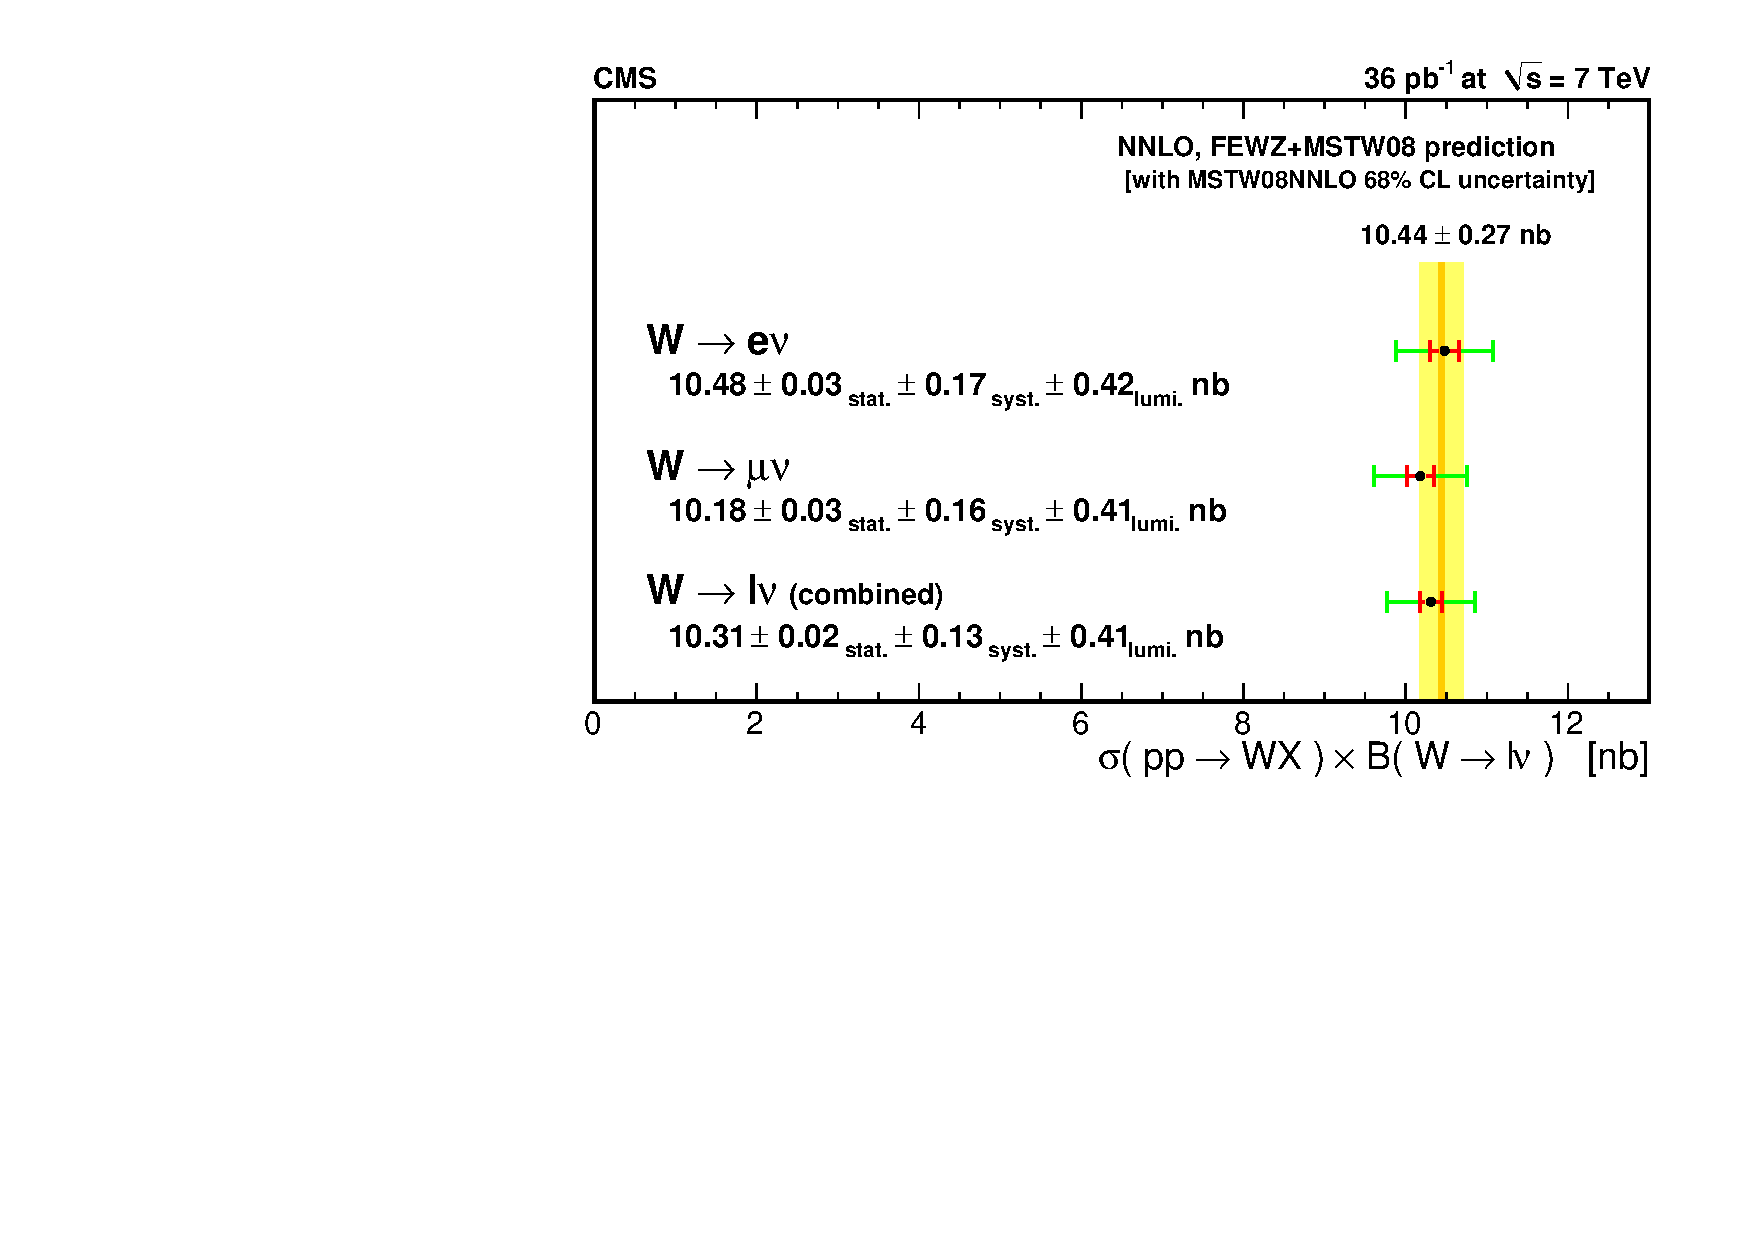
\includegraphics[width=0.495\textwidth]{figs/Results_W.pdf}
  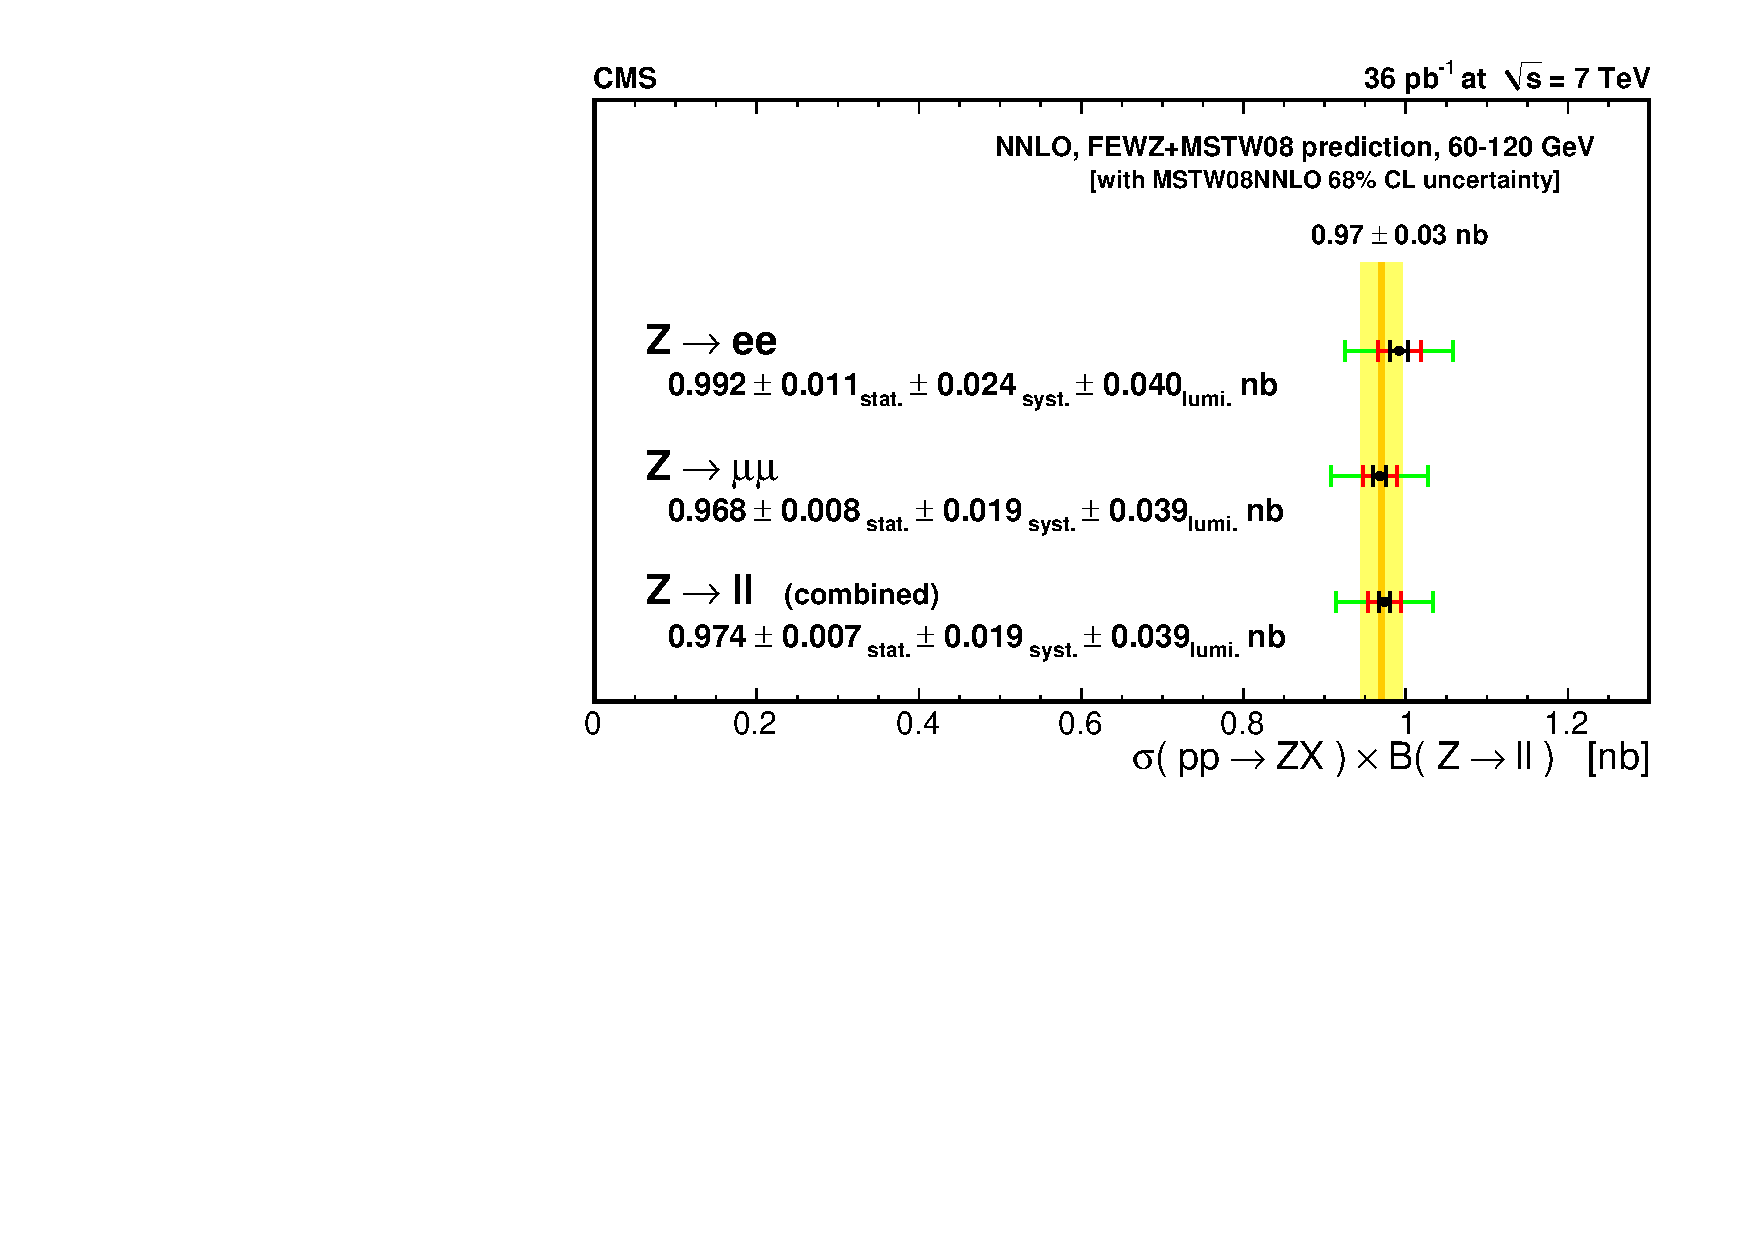
\includegraphics[width=0.495\textwidth]{figs/Results_Z.pdf}
\caption[.]{\label{fig:WZ_LEPstylePlots}
Summary of the $\Wo$ and $\Zo$ production cross section times branching ratio measurements.
Measurements in the electron and muon channels, and combined, are compared to the
theoretical predictions (yellow band) computed at the NNLO in QCD with recent PDF sets.
Statistical uncertainties are represented as a black error bars, while the red error bars also include systematic uncertainties,
and the green error bars also include luminosity uncertainties.
}
\end{center}
\end{figure}


\begin{figure}[htbp]
\begin{center}
  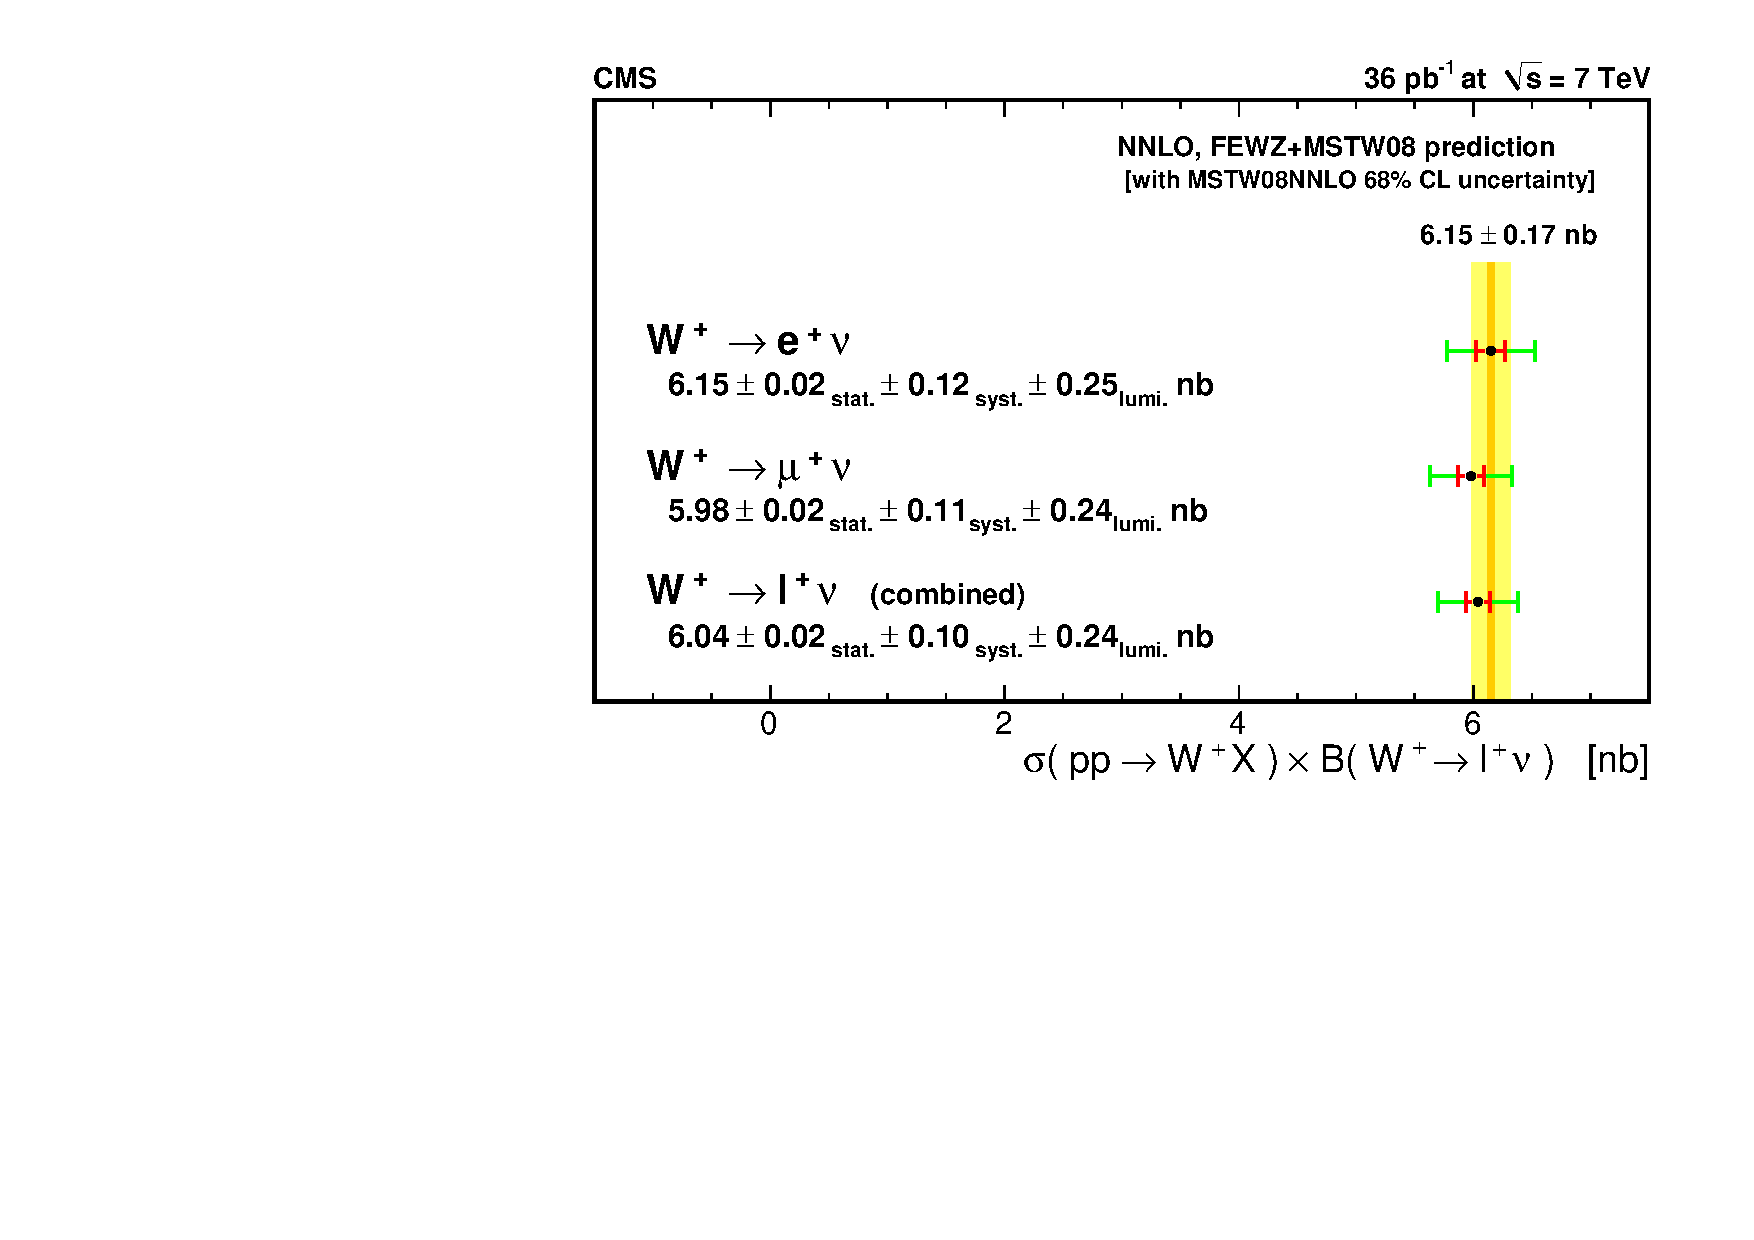
\includegraphics[width=0.495\textwidth]{figs/Results_W_plus.pdf}
  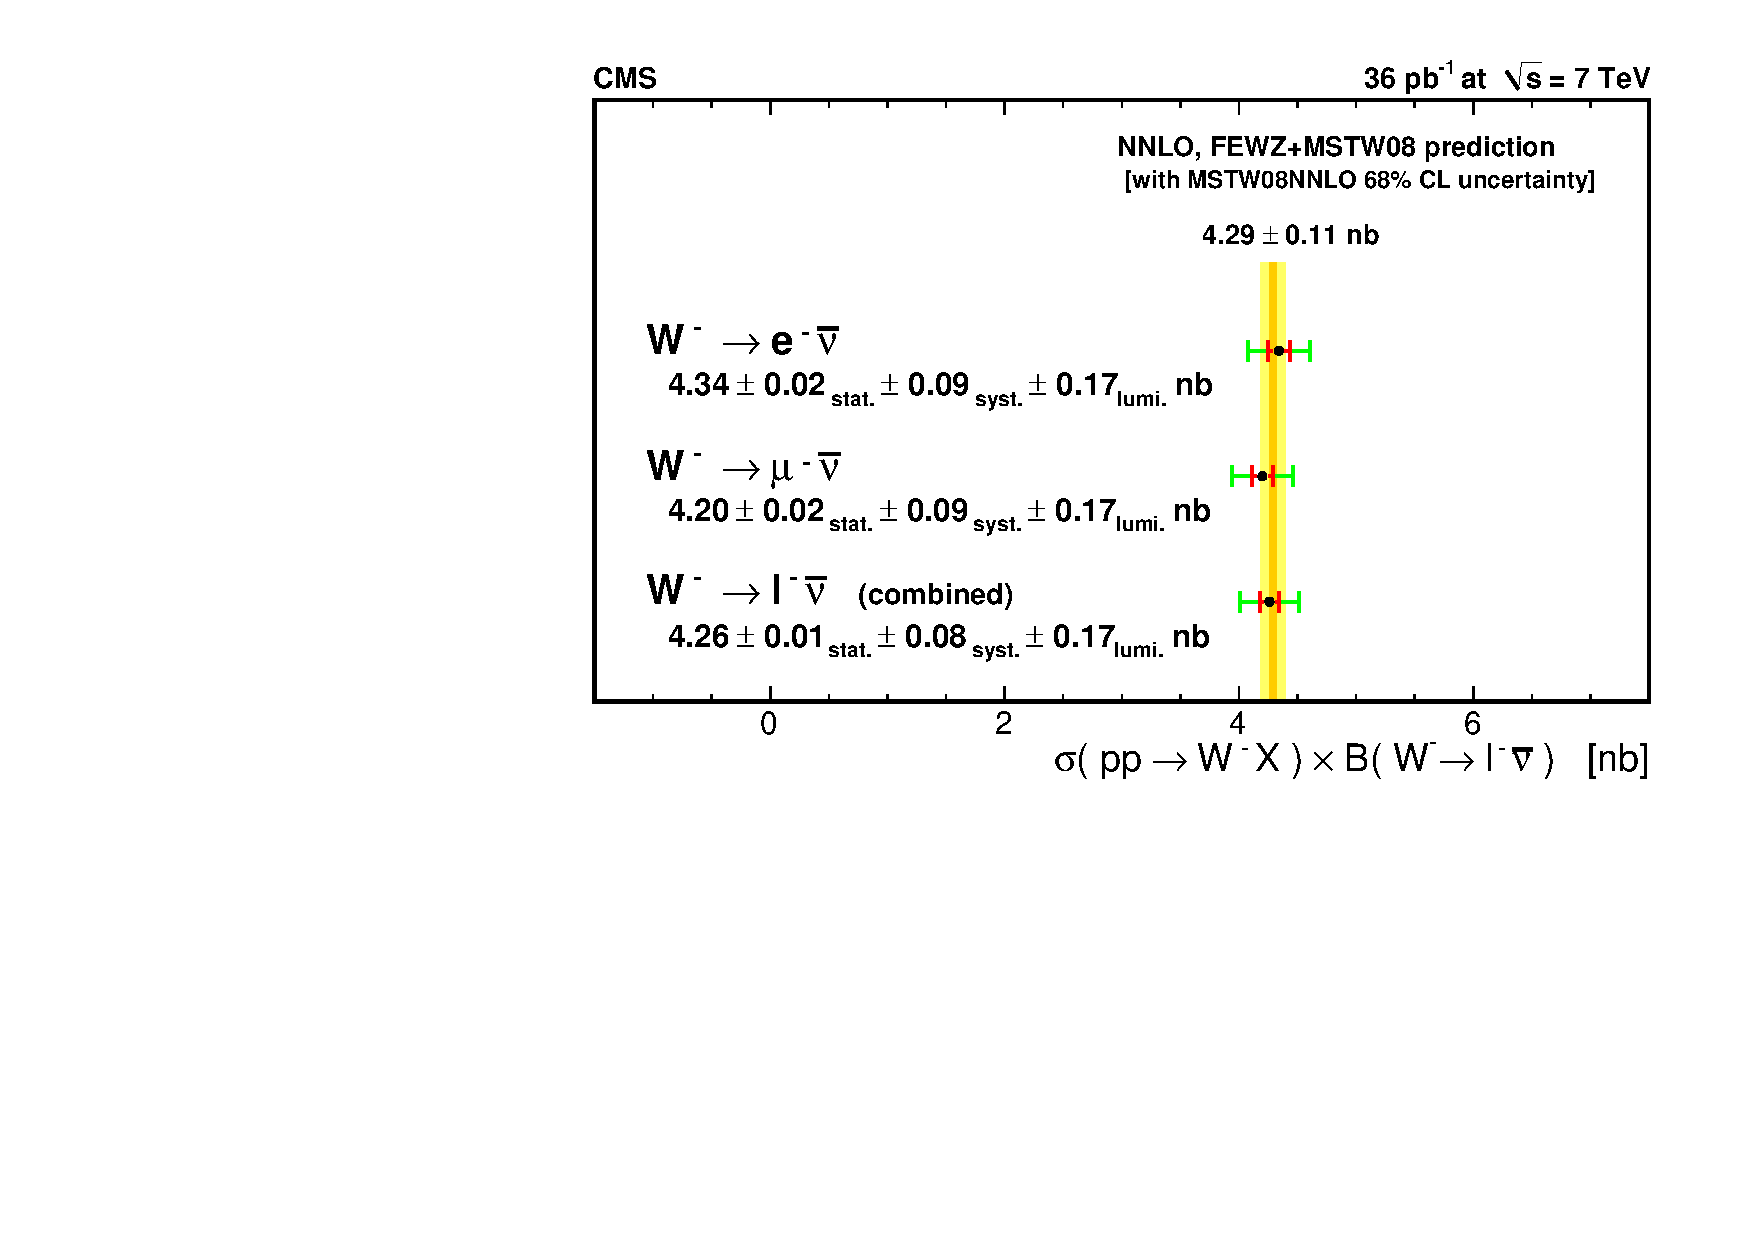
\includegraphics[width=0.495\textwidth]{figs/Results_W_minus.pdf}
\caption[.]{\label{fig:WPM_LEPstylePlots}
Summary of the $\Wp$ and $\Wm$ production cross section times branching ratio measurements.
Measurements in the electron and muon channels, and combined, are compared to the
theoretical predictions computed at the NNLO in QCD with recent PDF sets.
Statistical uncertainties are negligible in this plot; the red error bars represent systematic uncertainties,
and the green error bars also include luminosity uncertainties.
}
\end{center}
\end{figure}

\begin{figure}[htbp]
\begin{center}
  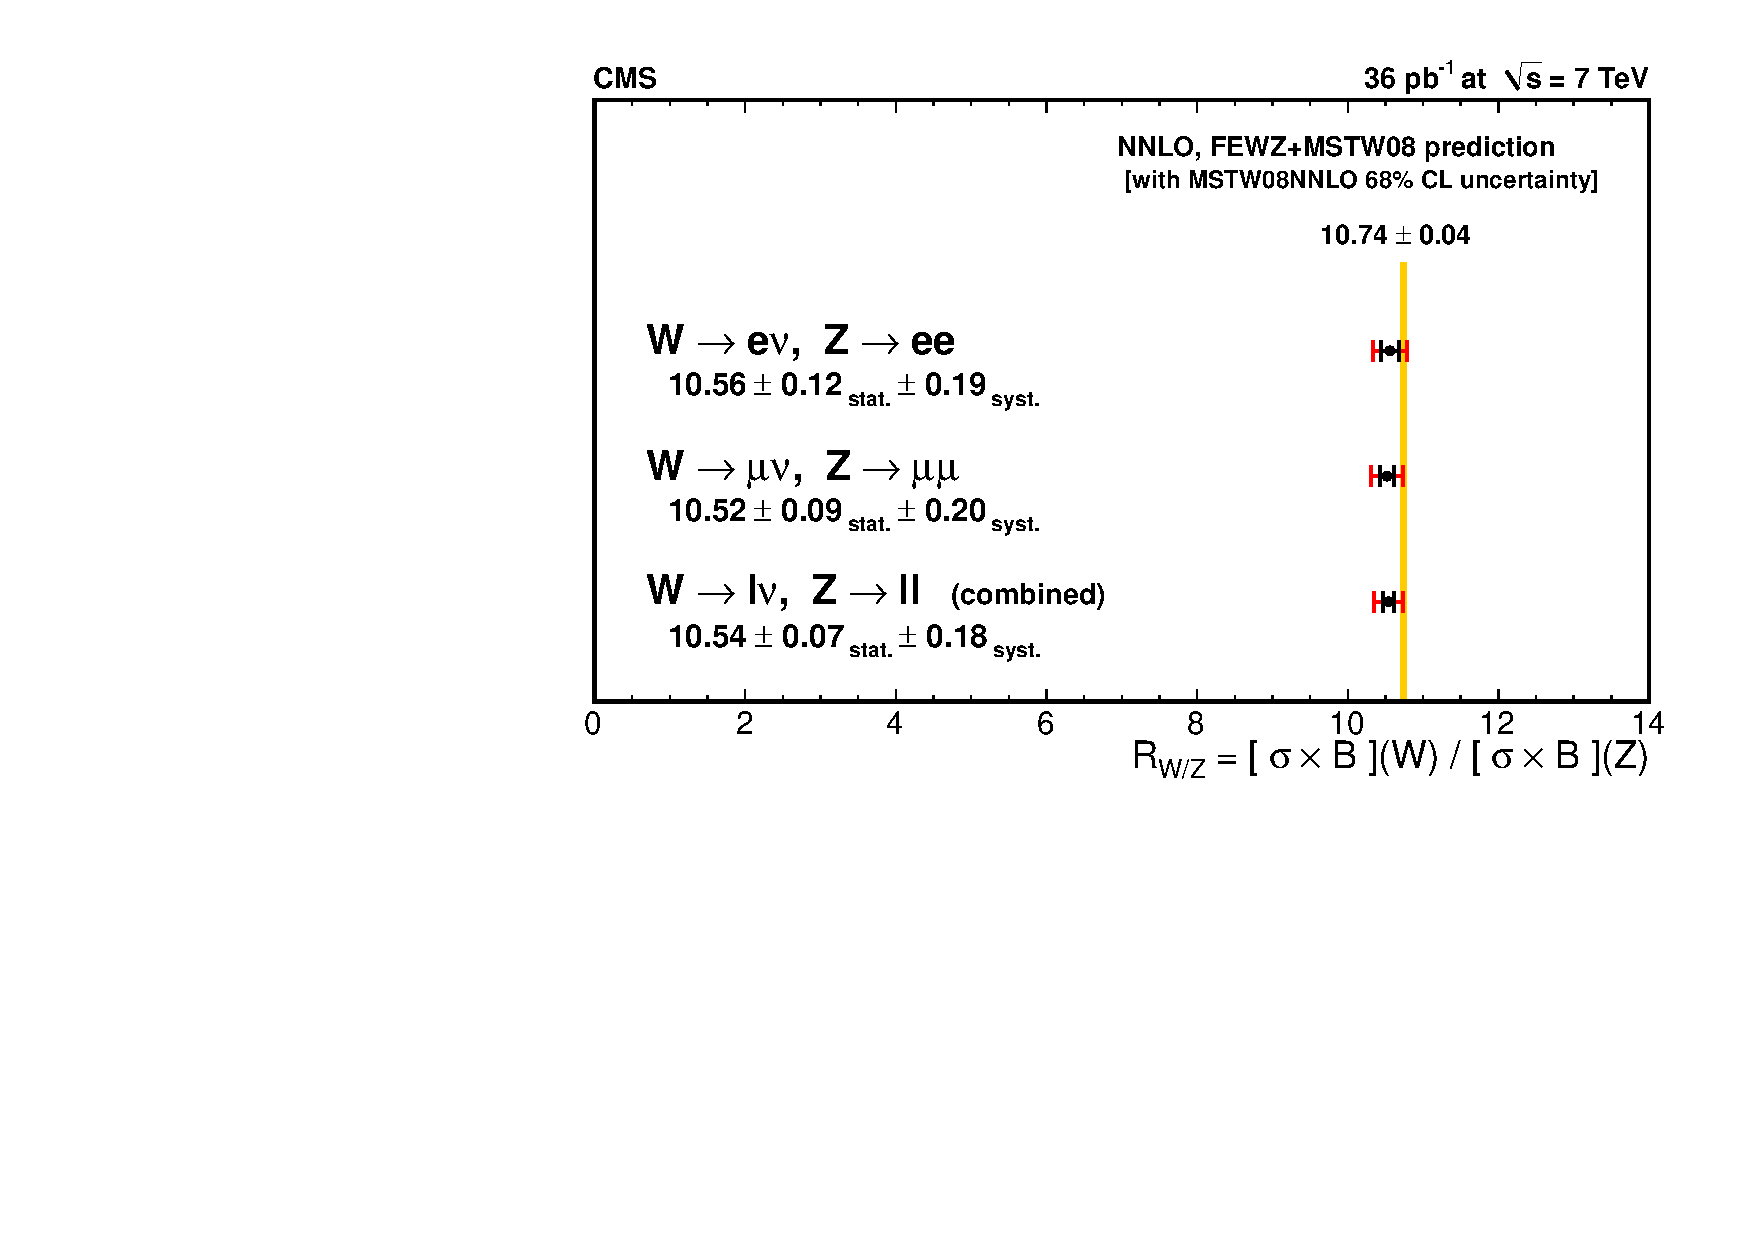
\includegraphics[width=0.495\textwidth]{figs/Results_R_WZ.pdf}
  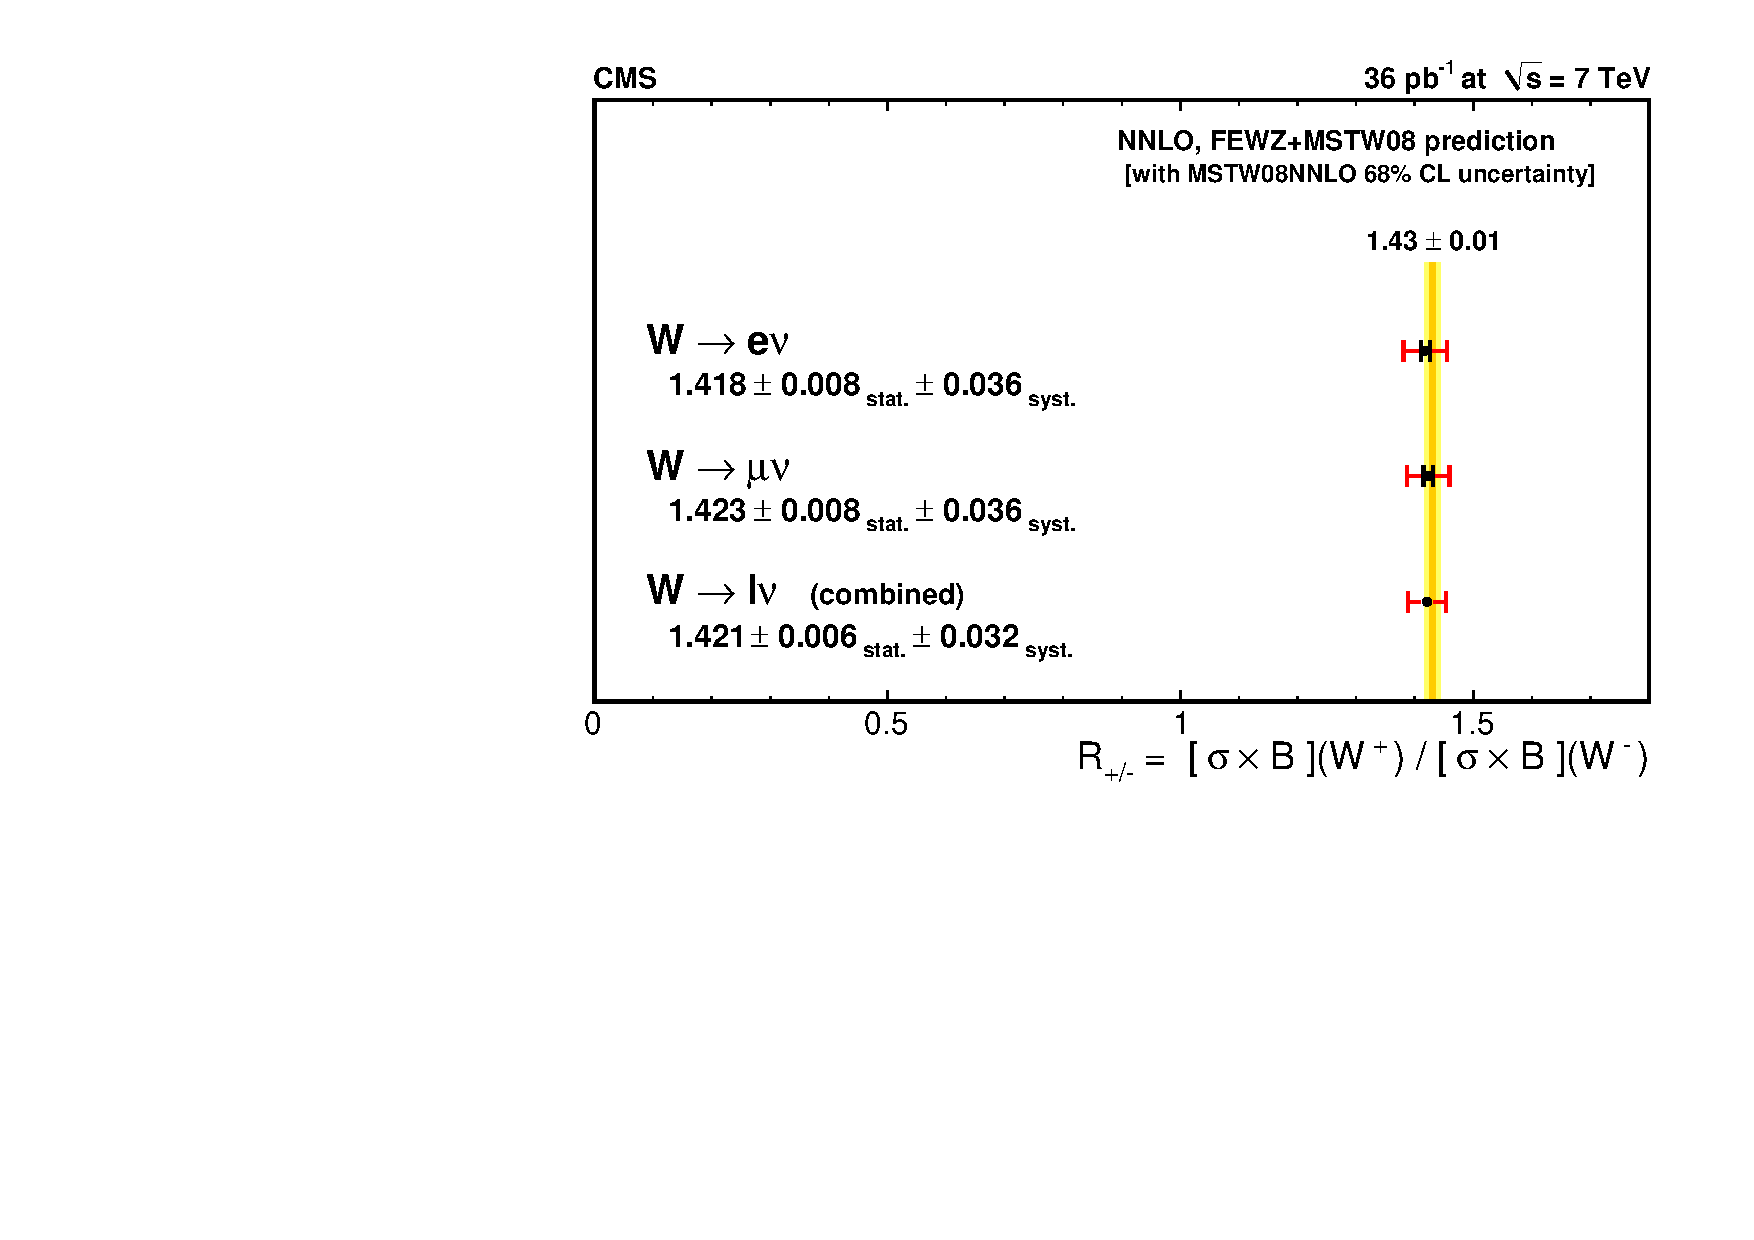
\includegraphics[width=0.495\textwidth]{figs/Results_R_WpWm.pdf}
\caption[.]{\label{fig:R_LEPstylePlots}
Summary of the measurements of the ratios of W to Z and $\Wp$ to $\Wm$ production cross sections.
Measurements in the electron and muon channels, and combined, are compared to the
theoretical predictions computed at the NNLO in QCD with recent PDF sets.
Statistical uncertainties are represented as a black error bars, while the red error bars also include systematic uncertainties.
Luminosity uncertainties cancel in the ratios.
}
\end{center}
\end{figure}

\begin{figure}
\begin{center}
  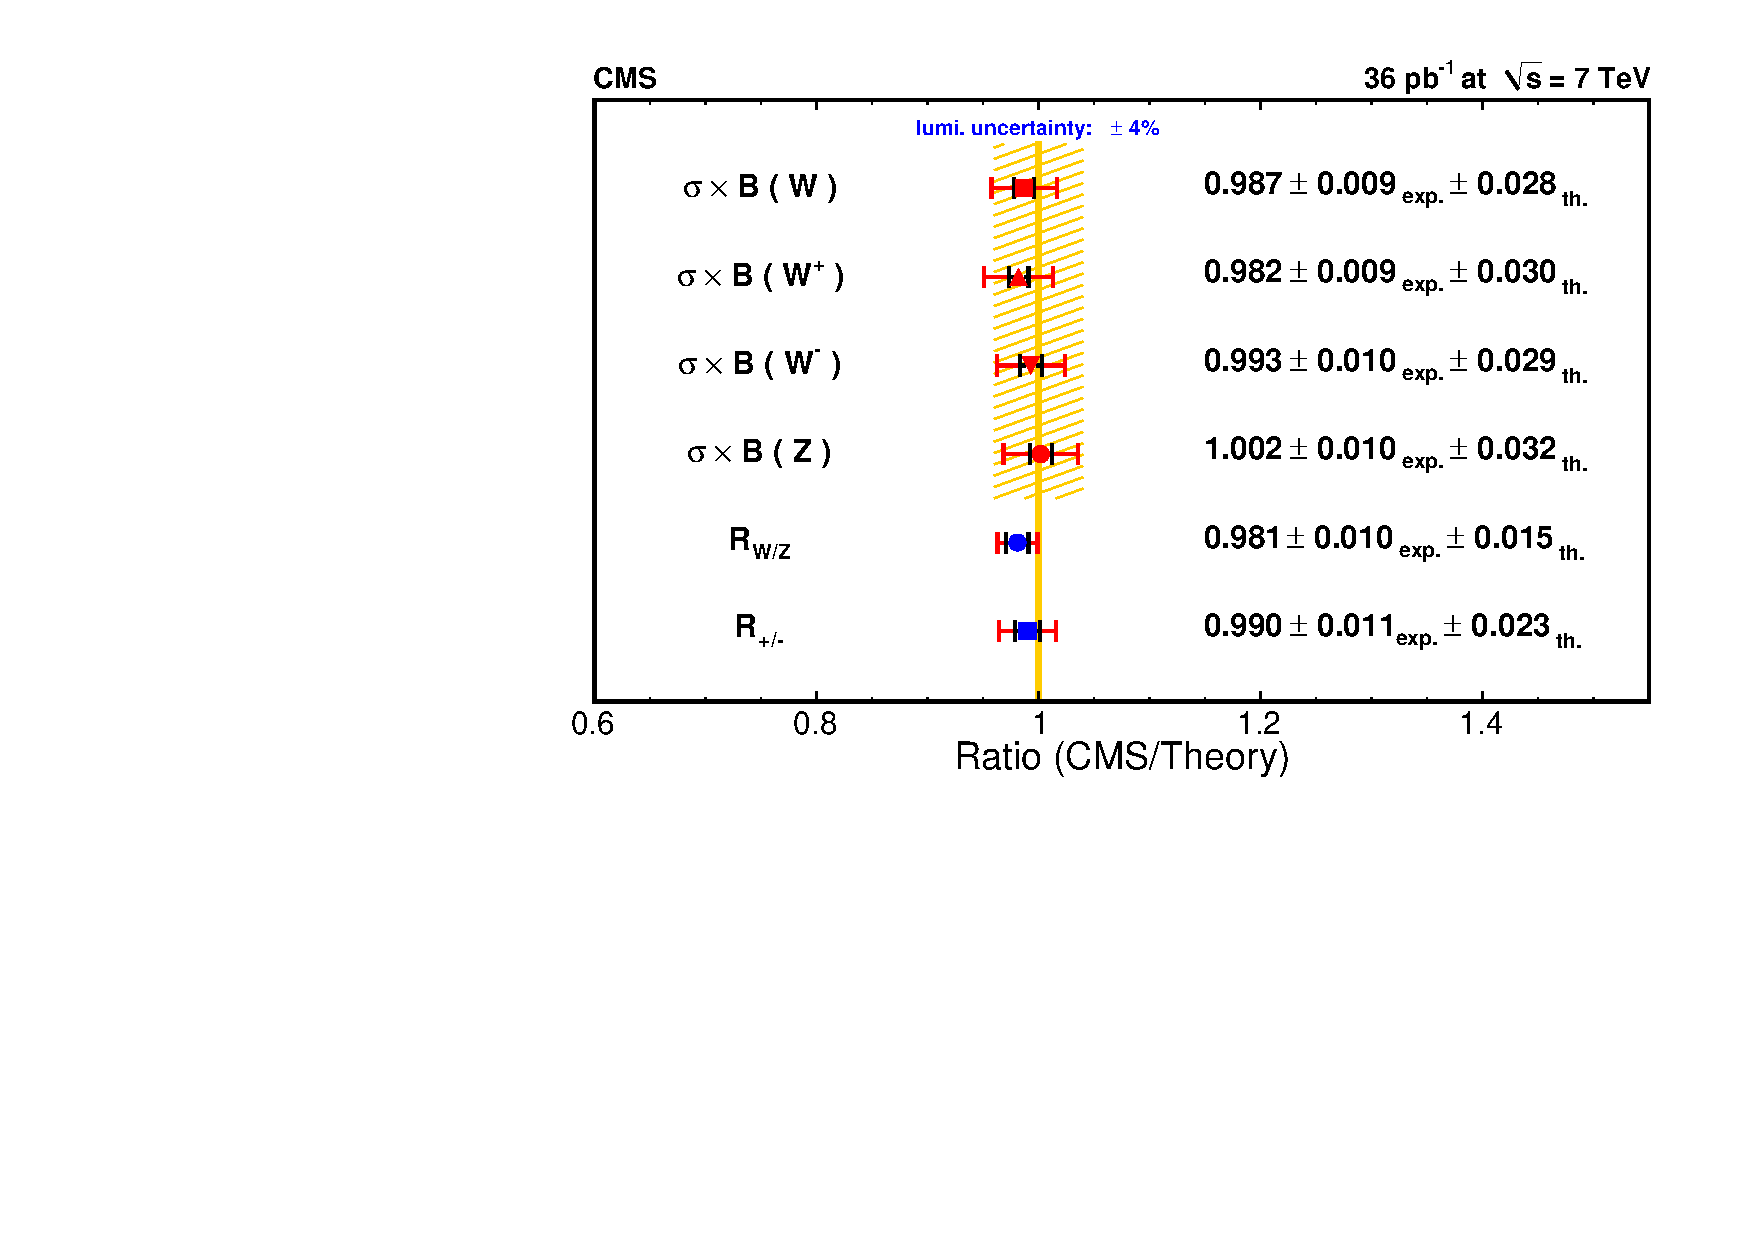
\includegraphics[width=0.7\textwidth]{figs/Results_ratioTheory.pdf}
\caption[.]{\label{fig:RatioCMSTHY}
Summary of ratios of the CMS measurements to the theoretical predictions.
The experimental uncertainties are represented as black error bars, while the
red error bars also include the combining of theoretical uncertainties
on the predictions and measured quantities. The yellow band around the vertical yellow line at one
represent the luminosity uncertainty (4\%) that affects the cross-section measurements.
}
\end{center}
\end{figure}

\begin{table} %
\begin{center}
\caption[.]{ Summary of ratios of CMS measurements to the theoretical predictions. 
The experimental uncertainty (exp.) is computed as the sum in quadrature of
the statistical and experimental systematic uncertainties, aside from the uncertainty on the 
integrated luminosity, which is shown separately.}
%integrated luminosity, which is shown separately in Fig.~\ref{fig:RatioCMSTHY}.}
\begin{tabular}{|l|c|}
\hline
Quantity & Ratio (CMS/Theory) \\
\hline\hline
$\SIGBRSHORT{\Wpm}$   & $\RATCMSTHYWI$ \\
$\SIGBRSHORT{\Wp}$     & $\RATCMSTHYWP$ \\
$\SIGBRSHORT{\Wm}$     & $\RATCMSTHYWM$ \\
$\SIGBRSHORT{\Zo}$       & $\RATCMSTHYZ$  \\
$\SIGBRSHORT{\Wo}/\SIGBRSHORT{\Zo}$     & $\RATCMSTHYWZ$ \\
$\SIGBRSHORT{\Wp}/\SIGBRSHORT{\Wm}$ & $\RATCMSTHYWW$ \\
\hline
\end{tabular}
\label{tab:RatioCMSTHY}
\end{center}
\end{table}


Figure~\ref{fig:WZsigmas} shows the CMS W and Z cross section measurements together
with measurements at lower center-of-mass energy hadron colliders.
The predicted increase of the cross sections with center of mass energy is confirmed
by our measurements.

\begin{figure}
\begin{center}
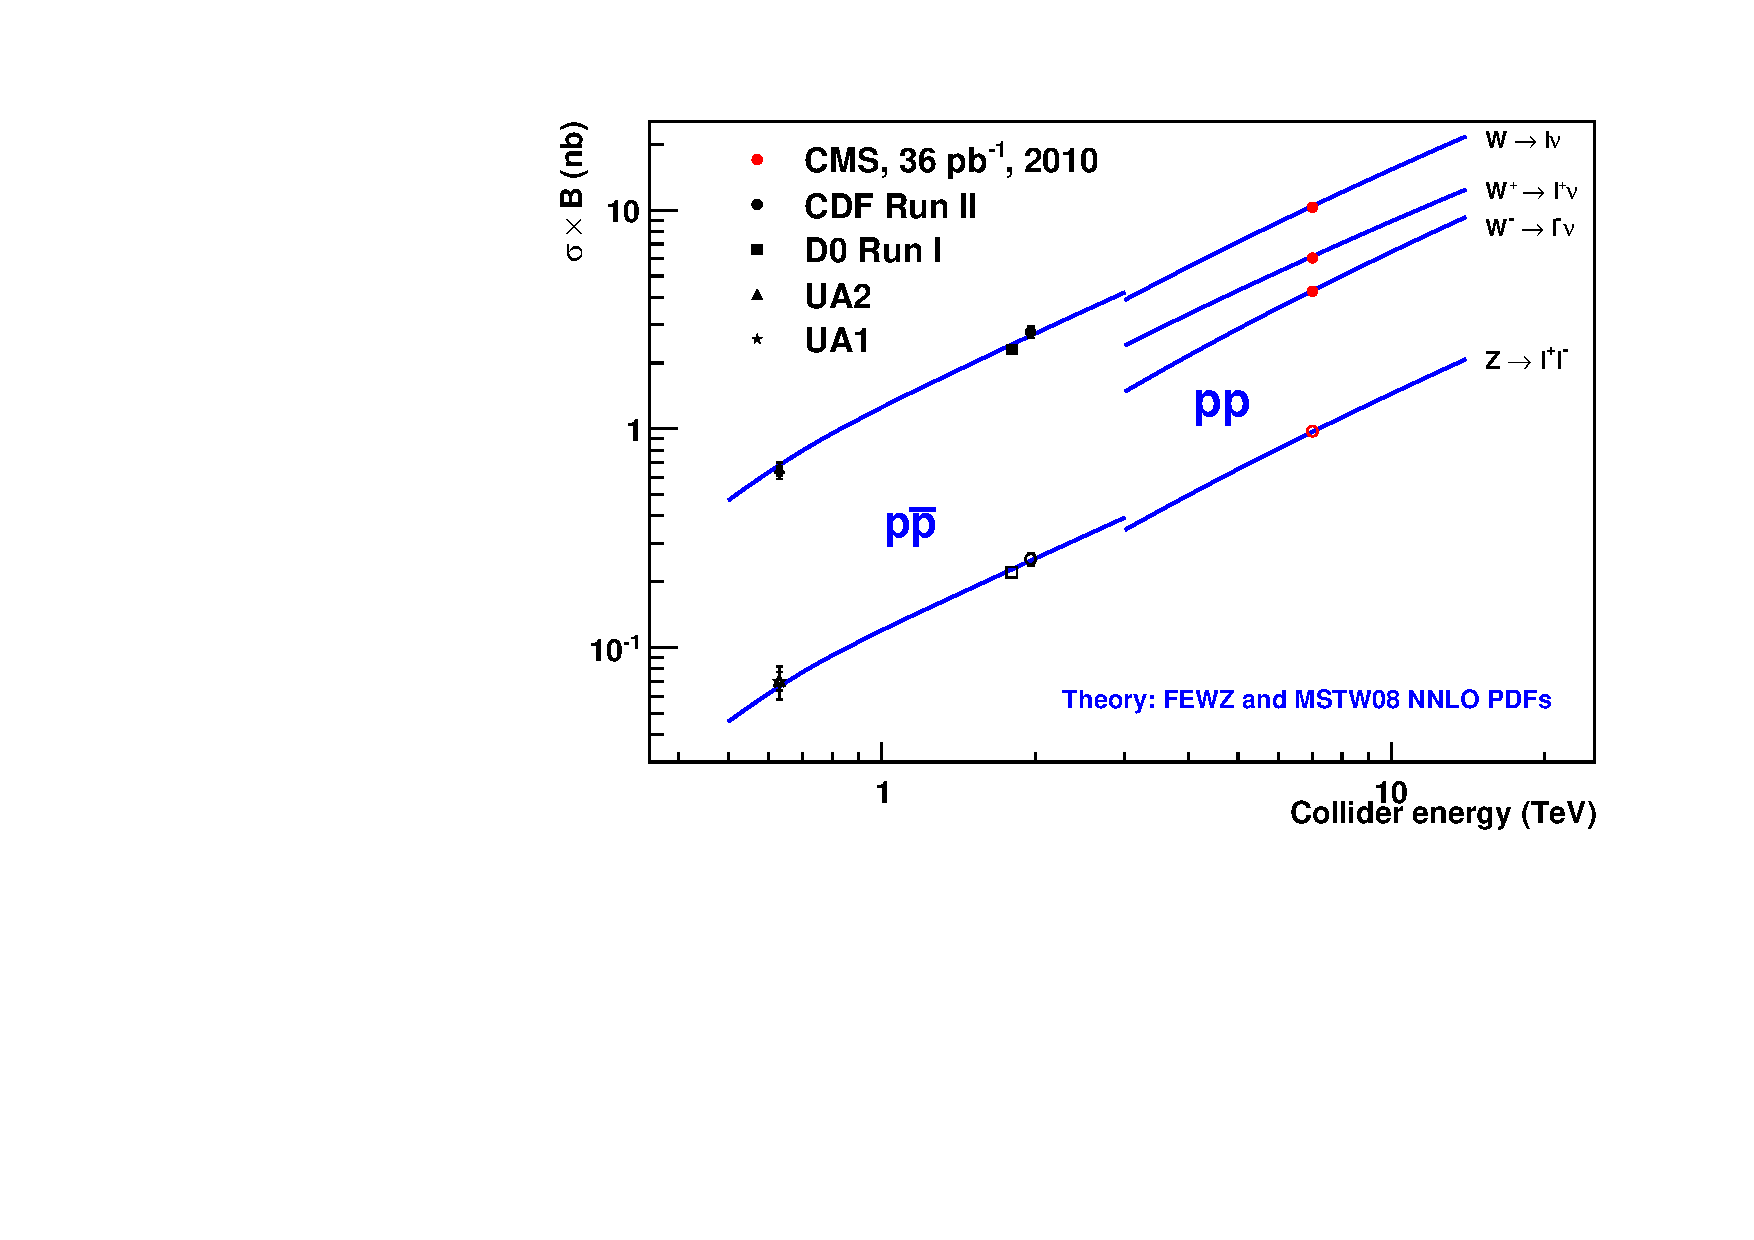
\includegraphics[width=0.8\textwidth]{figs/WZsigmas.pdf}
%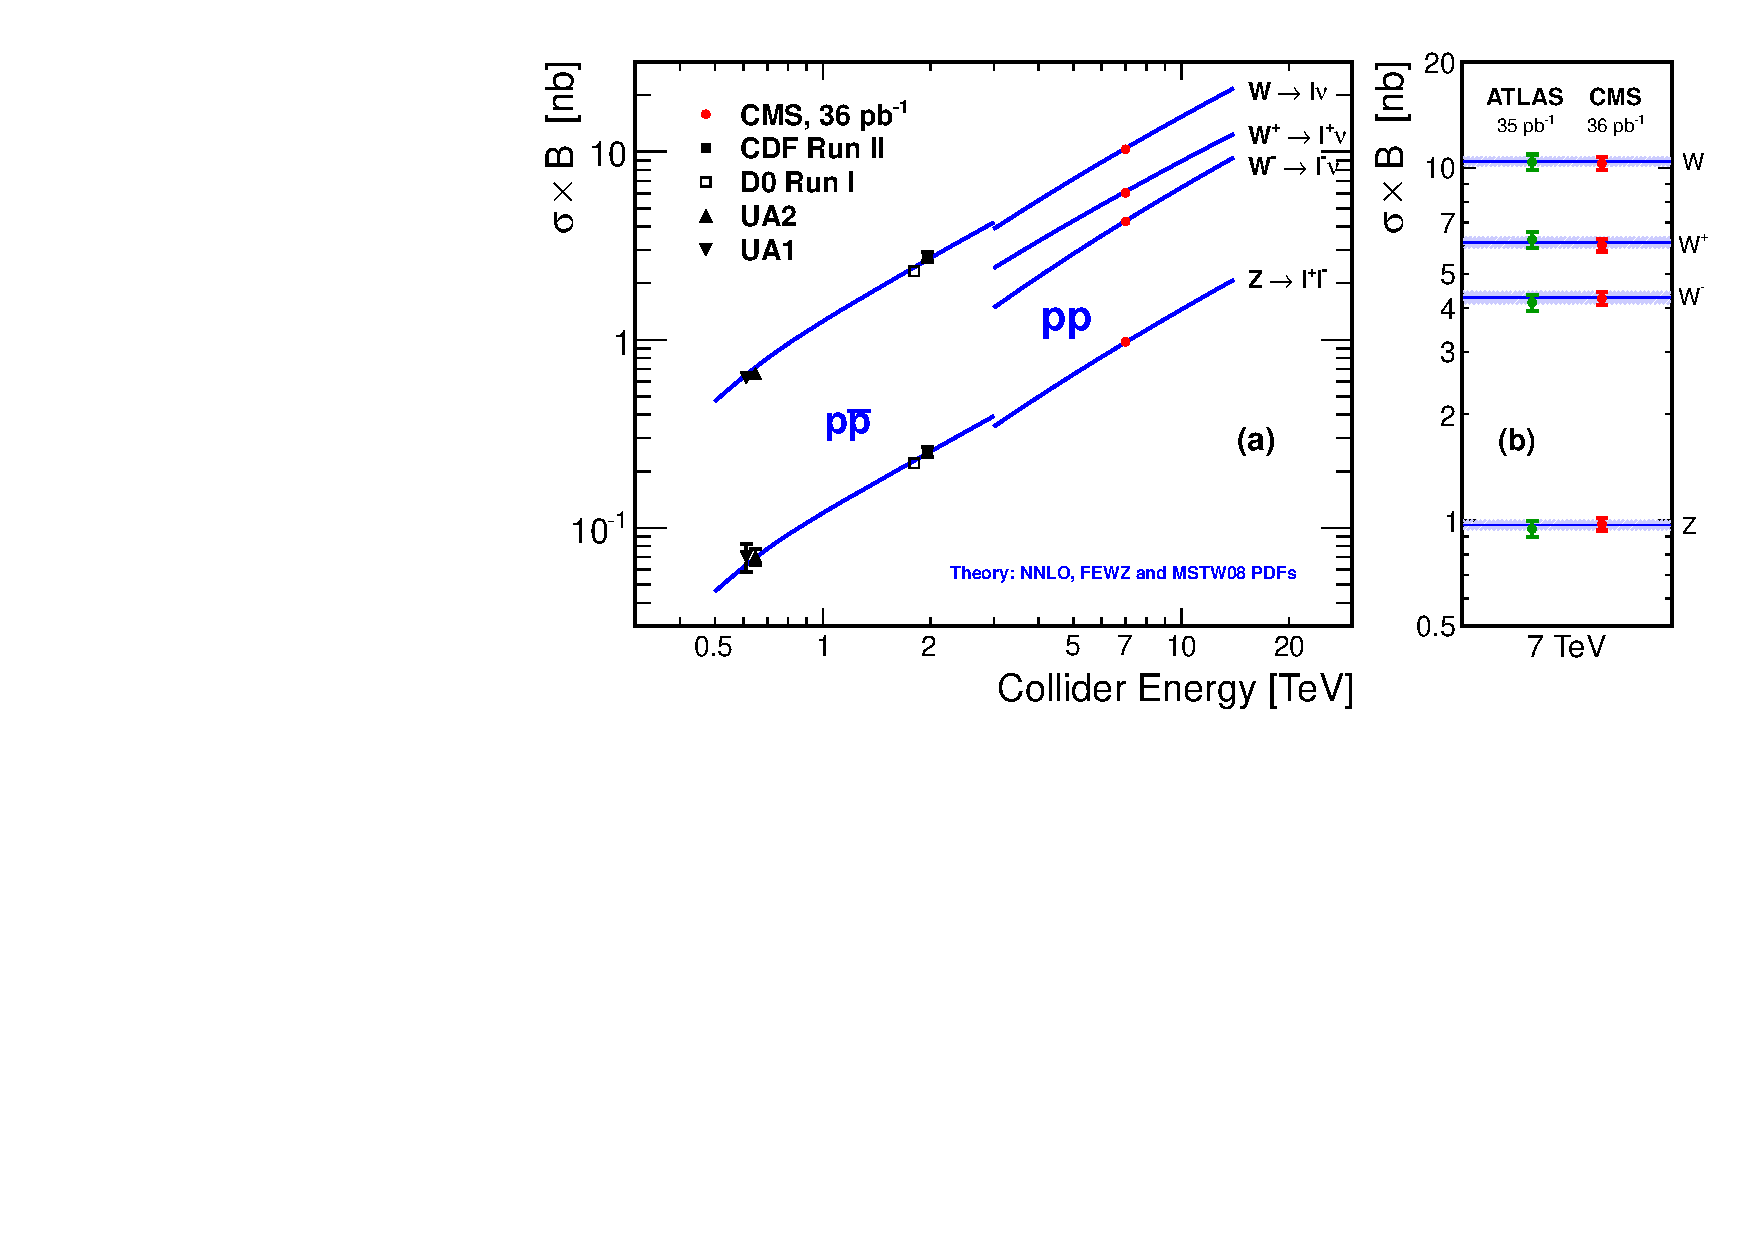
\includegraphics[width=1\textwidth]{figs/atlas-cms.pdf}
\caption[.]{\label{fig:WZsigmas}
Measurements of inclusive W and Z production cross sections
times branching ratios as a function of center-of-mass energy for CMS and experiments
at lower-energy colliders. The lines are the NNLO theory predictions.
%The solid symbols represent
%$\sigma( \pp \to \Wo X)\times {\cal B}(\Wo\rightarrow\ell\nu)$ and the
%hollow symbols, $\sigma(\pp\to\Zo X)\times {\cal B}(\Zo\rightarrow\ell^+\ell^-)$.
%Theoretical predictions are shown as blue lines.
%(b) A comparison with the latest preliminary ATLAS results with 35~pb$^{-1}$ from
%Ref.~\cite{WZATLAS:2011}
%is shown. The blue lines show the theoretical predictions with their uncertainty.
%CMS (red, four points on the right side) and ATLAS (green, four point on the left side) measurements are
%shown with the total experimental, theoretical
%and luminosity uncertainties. The luminosity uncertainties amount to 3.4\% for ATLAS and 4\% for CMS.
}
\end{center}
\end{figure}





\par
Table~\ref{tab:res-restricted-xsections} reports the cross sections 
as measured within the fiducial and kinematic acceptance, thereby eliminating the PDF uncertainties
from the results. In effect, these
uncertainties are transferred to the theoretical predictions,
allowing for a cleaner separation of experimental and
theoretical uncertainties.
For each channel the fiducial and kinematic acceptance
is defined as the fraction of events with lepton $\pt$ greater than $25~\GeV$
($20~\GeV$ for $\Zmm$), including no final-state QED radiation,
and with pseudorapidity in the range $|\eta|<2.5$ for electrons
and $|\eta|<2.1$ for muons.
Table~\ref{tab:res-restricted-ratios} reports the 
ratios of cross sections for $\Wo$ and $\Zo$ production and for $\Wo^+$ and $\Wo^-$ production
within the fiducial and kinematic acceptances, separately for electron
and muon channels.


\begin{table}[hbt] %
\begin{center}
\caption[.]{Summary of production cross section measurements and ratios
in restricted fiducial and kinematic acceptances. The $\pt$ and $|\eta|$
requirements restricting the acceptance for electrons and muons,
and the resulting acceptance values, are also given. The quoted uncertainties on
the acceptances (evaluated without FSR effect) are due to the PDF uncertainties.
\label{tab:res-restricted-xsections} }
\begin{tabular}{|l|r|c|c|}
\hline
\multicolumn{1}{|c|}{Channel} &
\multicolumn{1}{c|}{$\sigma \times {\cal B}$ in acceptance $A$ (nb)}&
\multicolumn{2}{c|}{$A$}
\\
\hline
\hline
$\Wen$  & %\WEISIGBRXGD
{\footnotesize $5.688 \pm 0.016\,\mathrm{(stat.)} \pm 0.090\,\mathrm{(syst.)} \pm 0.228\,\mathrm{(lumi.)}$} & $0.543 \pm 0.003$ & \\
$\Wpen$ & % \WEPSIGBRXGD
{\footnotesize $3.404 \pm 0.012\,\mathrm{(stat.)} \pm 0.064\,\mathrm{(syst.)} \pm 0.136\,\mathrm{(lumi.)}$} & $0.554 \pm 0.004$ & $\pt>25\GeV$  \\
$\Wmen$ & %\WEMSIGBRXGD
{\footnotesize $2.284 \pm 0.010\,\mathrm{(stat.)} \pm 0.040\,\mathrm{(syst.)} \pm 0.091\,\mathrm{(lumi.)}$} & $0.527 \pm 0.006$ & $|\eta|<2.5$   \\
$\Zee$  & %\ZEESIGBRXGD
{\footnotesize $0.452 \pm 0.005\,\mathrm{(stat.)} \pm 0.010\,\mathrm{(syst.)} \pm 0.018\,\mathrm{(lumi.)}$} & $0.456 \pm 0.004$ & \\
\hline \hline
$\Wmn$  & {\footnotesize \WMISIGBRXGD }
%$\pm \mathrm{(stat.)} \pm \mathrm{(syst.)} \pm \mathrm{(lumi.)}$
& $0.465 \pm 0.004$ & {\multirow{3}{*}{\begin{tabular}{c}$\pt>25\GeV$\\$|\eta|<2.1$ \end{tabular}}} \\
$\Wpmn$ & {\footnotesize \WMPSIGBRXGD }
%$\pm \mathrm{(stat.)} \pm \mathrm{(syst.)} \pm \mathrm{(lumi.)}$
& $0.471 \pm 0.004$ &   \\
$\Wmmn$ & {\footnotesize \WMMSIGBRXGD }
%$\pm \mathrm{(stat.)} \pm \mathrm{(syst.)} \pm \mathrm{(lumi.)}$
& $0.457 \pm 0.007$ &   \\
\hline%\cline{4-4}
{\multirow{2}{*}{$\Zmm$}}  & %\ZMMSIGBRXGD
{\multirow{2}{*}{{\footnotesize $0.396 \pm 0.003\, \mathrm{(stat.)} \pm 0.007\, \mathrm{(syst.)} \pm 0.016\, \mathrm{(lumi.)}$}}} &
{\multirow{2}{*}{$0.409 \pm 0.005$}} & $\pt>20\GeV$\\
 & & & $|\eta|<2.1$ \\
\hline
\end{tabular}
\end{center}
\end{table}

\begin{table}[hbt] %
\begin{center}
\caption[.]{Ratios of cross sections for $\Wo$ and $\Zo$ production and for $\Wo^+$ and $\Wo^-$ production
in restricted fiducial and kinematic acceptances for electron and muon channels.
The $\pt$ and $|\eta|$ requirements are the same as those quoted in Table~\ref{tab:res-restricted-xsections}.
\label{tab:res-restricted-ratios} }
\begin{tabular}{|l|r|r|}
\hline
\multicolumn{1}{|c|}{Channel} &
\multicolumn{1}{|c|}{Ratio of $\sigma\times{\cal B}$ in acceptances} &
\multicolumn{1}{|c|}{$A$ ratio} \\
\hline
\hline
$\Wo/\Zo\, (\mathrm{e})$  &  $12.58 \pm 0.14\,\mathrm{(stat.)} \pm 0.21\,\mathrm{(syst.)}$ & $0.839\pm 0.005$ \\
$\Wo^+/\Wo^-\, (\mathrm{e})$  &  $1.490 \pm 0.009\,\mathrm{(stat.)} \pm 0.029\,\mathrm{(syst.)}$ &$0.952\pm 0.015$ \\
\hline\hline
$\Wo/\Zo\, (\mu)$  &  $11.95 \pm 0.10\,\mathrm{(stat.)} \pm 0.20\,\mathrm{(syst.)}$& $0.880\pm 0.008$  \\
$\Wo^+/\Wo^-\, (\mu)$  &  $1.466 \pm 0.008\,\mathrm{(stat.)} \pm 0.023\,\mathrm{(syst.)}$ & $0.971\pm 0.018$ \\
\hline
\end{tabular}
\end{center}
\end{table}

\subsection{\texorpdfstring{Extraction of ${\cal B}(\Wln)$ and $\Gamma(\Wo)$}{Extraction of B(W->l n) and Gamma(W)}}
\label{sec:Gamma_W}

The precise value of the ratio of the W and Z cross sections
obtained from the combination of the measurements in the electron
and muon final states can be used to determine the SM
parameters ${\cal B}(\Wln)$ and $\Gamma(\Wo)$.

The ratio of W and Z cross sections can be written as
\begin{displaymath}
  R = \frac{\sigma(\pp \rightarrow \Wo X)}{\sigma(\pp \rightarrow \Zo X)}\,\,
  \frac{{\cal B}(\Wln)}{{\cal B}(\Zll)}\,.
\end{displaymath}


In order to estimate the value of ${\cal B}(\Wln)$
the predicted ratio of the W and Z production cross sections and the
measured value of the ${\cal B}(\Zll)$ are needed.
The NNLO prediction of the ratio, based on the MSTW08 PDFs, is $\sigma_\Wo$/$\sigma_\Zo$ = 3.34 $\pm$ 0.08.
The current measured value for ${\cal B}(\Zll)$ is 0.033658$\pm$0.000023
~\cite{PDG}. Those values lead to an indirect estimation of
\begin{displaymath}
{\cal B}(\Wln) = 0.106 \pm 0.003 \,,
\end{displaymath}
in agreement with the measured value, ${\cal B}(\Wln) = 0.1080 \pm 0.0009$~\cite{PDG}.

Using the SM value for the leptonic partial width,
$\Gamma(\Wln) = 226.6\pm 0.2$~MeV~\cite{GammaW-SM,GammaW-SM-New},
an indirect measurement of the total $\Gamma(\Wo)$ can be obtained through the formula
\begin{displaymath}
  {\cal B}(\Wln) = \frac{\Gamma(\Wln)}{\Gamma(\Wo)}\,.
\end{displaymath}

Based on the above values we obtain
\begin{displaymath}
\Gamma(\Wo) = 2144 \pm 62 ~~\mathrm{MeV}  \,.
\end{displaymath}

The SM prediction is 2093 $\pm$ 2 MeV~\cite{GammaW-SM-New} and the world average of experimental
results is 2085 $\pm$ 42 MeV~\cite{PDG}. The indirect measurement of $\Gamma(\Wo)$ is in good agreement
with the world average and the theoretical prediction, as well as other published measurements.



